\document[./main_hagedorn.tex]{subfiles}
\usepackage{pgfplots} % loads tikz which loads pgf
\usepackage{adjustbox}
\begin{document}
%\begin{adjustbox}{left}
\vspace{-2cm}
\begin{tikzpicture}[scale=1.5]
  \centering
\begin{pgfinterruptboundingbox}
  \coordinate (A) at (3,-0.25);
  \coordinate (P) at (0,2);

  \draw (0:2cm)   arc[radius=2cm,start angle=0,end angle=180]
        (210:2cm) arc[radius=2cm,start angle=210,end angle=330];
  \draw (180:2cm) arc[x radius=2cm, y radius=0.5cm, start angle=180,end angle=360];

  \draw [dashed] (210:2cm)
        arc[start angle=210,delta angle=-30,radius=2cm]
        arc[start angle=180,delta angle=-180,x radius=2cm,y radius=0.5cm]
        arc[start angle=0,delta angle=-30,radius=2cm];

  \draw [dashed] (80:2cm and 0.5cm) -- (260:2cm and 0.5cm);
  \draw [dashed] (150:2cm) coordinate(ul) -- (30:2cm) coordinate(ur);

  \draw (-4.5,-1) -- (3.5,-1) -- (4.5,1) node[anchor=south east] {\scriptsize$ z=0 $} -- (ur) (ul) -- (-3.5,1) -- (-4.5,-1);

  \draw (A) -- (P) coordinate[pos=0.47](B);
  \path (A) node[circle, fill, inner sep=1pt, label=below:{\scriptsize$ P(x,y,0) $}]{};
  \path (B) node[circle, fill, inner sep=1pt, label=left:{\scriptsize$ (\xi,\eta,\zeta) $}]{};
  \path (P) node[circle, fill, inner sep=1pt, label=above:{\scriptsize$ (0,0,1) $}]{};
  \draw [dashed] (-2,0) -- (2,0);
\end{pgfinterruptboundingbox}  
%\path[use as bounding box] ([yshift=-8mm]current axis.south west) rectangle (current axis.north east);
\end{tikzpicture}
%\end{adjustbox}
\end{document}
